\documentclass[A4,12pt]{article}
\usepackage{geometry}
\usepackage{multicol}
\usepackage{lipsum}
\usepackage{changepage}
\usepackage{graphicx}
\graphicspath{  }
\usepackage{booktabs}
\usepackage{cite}
\usepackage{float}
\usepackage{hyperref}
\usepackage[font={small,it}]{caption}
\usepackage[english]{babel}
\usepackage{fancyhdr}

\graphicspath {{figures/}}

\setlength{\headheight}{15pt}

\pagestyle{fancy}
\fancyhf{}
\lhead{\textbf{Version:} 1.0  \textbf{Revision:} 05/03/18}
\rhead{\thepage}
\lfoot{Mitch Frand}
\rfoot{\textit{Mu2e: University of Minnesota}}

\renewcommand{\footrulewidth}{1pt}


\begin{document}
\begin{titlepage}
	\centering
	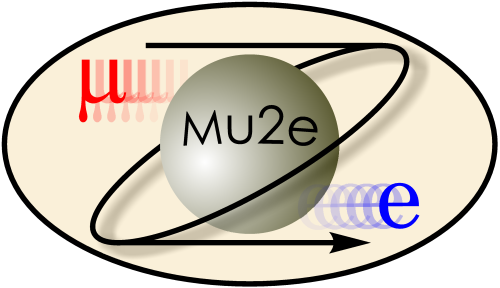
\includegraphics[width=0.5\textwidth]{mu2e_logo_oval.png}\par\vspace{2cm}
	{\scshape\LARGE Straw Cutting Standard Operating Procedure\par}
	\vspace{3cm}
	{\Large Mitch Frand\par}
	\vspace{3cm}
	{\large University of Minnesota\par}
 	\vspace{.5cm}
	{\large May 10, 2018\par}
	% Bottom of the page
	\vfill
	{Frand053@umn.edu\par}
\end{titlepage}

\clearpage
\setcounter{page}{2}
\newenvironment{myitemize} %adjust item spacing in lists to make smaller
{ \begin{itemize}
    \setlength{\itemsep}{4pt}
    \setlength{\parskip}{0pt}
    \setlength{\parsep}{0pt}     }
{ \end{itemize}                  } 

\section{Goal}
Straws on mu2e panels need to have precise dimensions to be used effectively.  Small errors in the cutting process can ruin straws.  The laser cutter, when used properly, is capable of quickly cutting the straws to their necessary lengths.  The purpose of this document is to demonstrate the proper procedure for cutting the straws safely and correctly using the AP LAZER SN2816.


\section{Equipment}
\begin{multicols}{2}
\begin{myitemize}
	\item Pallet with Mylar straws
	\item Form-fitting nitrile gloves
    \item AP LAZER SN2816
    \item Computer for uploading data 
    \item Rubber mats
    \item Laser cutter safety key
\end{myitemize}
\end{multicols}



\section{Risks and Dangers}
Always wear gloves while working with straws to keep them clean.  The AP LAZER SN2816 is a class four invisible laser.  Exposure to the eyes for as little as a microsecond will cause blindness.  Because of this, the laser is equipped with numerous safety features.  Be very careful to follow all steps in the procedure.  There is an emergency stop button located on the right side at the front end of the machine.  It should be used whenever the laser is in a position to cause harm to its users or itself.  To disengage the stop button it must be turned clockwise.  Never leave the laser cutter unattended and report unexpected behavior to a supervisor.





\section{Procedure}
	\subsection{Preparation}
\begin{enumerate}
	\item Before loading straws, cover them with rubber mats to secure them and prevent nudging.  		\item Then, facing the front of the laser, load a full pallet of straws.  Orient them such that the left side of the pallet has the longest straw position.  Line up the pallet flush against the white plastic guide and slide the pallet into the laser until the dowel pin nearer to you (Dowel pin holes are located at the front and back on the right side of the pallet) lines up with the hole on the laser.  Place a dowel pin in this hole to keep the pallet from sliding.  
    \item To turn the laser on, take the key out of the laser's dedicated toolbox and place it in the keyhole.  The keyhole is black and located next to the emergency stop button.  Turn the key to the"On" position.
    \item Confirm that the laser is set at the correct height by moving the laser head over the pallet.  To move the laser press the "esc" button on the laser panel twice.  Use the direction pad to navigate.  Using the height gauge tool, verify the laser is focused between the top surface of the straw and the middle of the straw. 
    \end{enumerate}
    \subsection{Cutting the Straws}
    \begin{enumerate}
    \item The laser cutter is controlled by a computer program called, "LaserCut 5.3".  This program can be found on the desktop under the name "LaserCut 2816".  Double click the icon to start the program.  The controls on the right side of the screen will be used to operate and communicate with the laser.
    \item To open a specific cutting file, go into the "file" menu and click 'open'.  A dialogue box will open and files can be added.  Once a chosen file is open, it must be uploaded into the laser.  To do this, click the download button at the bottom right of the screen.  Then click the "Del all" button and finally "Download current".  When the upload is complete, close out of the prompt box.
    \item Make sure the laser traces a path over the desired cutting region.  Press the "Run Box" button and make sure the laser is going over the anticipated cut region.  If the laser does not, try clicking the "Datum" button.  This will make the laser go back to its starting position in the top left corner of its work area.  Note: If the laser, at any time, tries to move beyond its work area (It will make a grinding noise), immediately hit the emergency stop and find help.  
    \item Do one final check by clicking the magnifying glass in the toolbar.  This will trace the cutting path with a red line.  If the path is incorrect, clear the simulated cuts by scrolling out and re-downloading the cut program.  Do not move on until the traced path is correct.
    \item To begin the cut, press the "Start" button on the LaserCut 5.3 panel.  This will initiate the cut.  The "Pause" button can be pressed to temporarily halt the cut.  The "Stop" button will stop the cut.  If the program is stopped in this way, it cannot restart from where it left off, but will restart the cut.
    \item If after running the program once the straws are not all cut you can rerun the program.  If two runs does not cut all the straws, consult a supervisor.
    \item When the first cut is done, remove the dowel pin and slide the pallet farther into the laser SLOWLY.  Stop sliding when the dowel pin closer to you aligns with the hole in the platform that is located within the workspace of the laser.  Realign the pallet with the white plastic guide and repeat the above steps to perform the cut.
    \item When finished, remove the pallet and turn the laser off by turning the key slot to "Off".  Return the key to its designated box.
    \end{enumerate}
    

\section{Cleanup}
\begin{enumerate}
	\item Turn off the laser by turning the key to "Off".  Place the key back in its designated spot in the toolbox.
    \item Remove the pallet and bring it to its next station.
    \item Clean up any easy to reach loose straw scraps
\end{enumerate}



\end{document}
